
\subsection{Permission and Rules Precedence}
It should be possible to override permissions and rules with another rule, but we need to establish priority among the permission and rules. 
For the overriding of the two to be relevant it they need to overlap in time which mean that the condition should use Timeperiod or True. Also if it is a rule then it should have an action with the name 'Cannot access controller', 'Access controller', 'Cannot access any controller' or 'Access any controller' to be relevant. 

We came to the conclusion that rules always have precedence over permissions. But if it is two rules it is a more complex precedence rules. First to determine the precedence we look at the action's name. See figure \ref{fig:precendence} where the precedence graph is shown. Notice that the precedence for 'Cannot access controller' and 'Access controller' can be either way depending on the condition. 
  
\begin{figure}
	\centering
		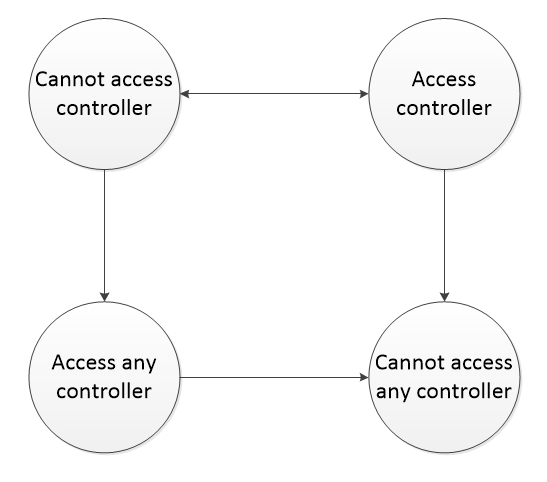
\includegraphics[width=1.00\textwidth]{images/precendence.jpg}
	\caption{Precedence of rules}
	\label{fig:precendence}
\end{figure}

When the condition determines the precedence we have different combinations:

\begin{itemize}
	\item If one is True and the other is Timeperiod then the rule with the Timeperiod has the higher precedence
	\item If both is True then Access controller has the precedence.
	\item If both is Timeperiod:
		\begin{itemize}
			\item If both is repeatable or non-repeatable then Access controller has the precedence
			\item If one is repeatable and the other is nonrepeatable then the rule with the nonrepeatable Timeperiod has the higher precedence.
		\end{itemize}
\end{itemize}

-----write more here------
